\section{Methodology}
Different tools helped us to understand a typical investment process to model the game best for a proper learning of the students, as described in section~\ref{sec:motivation}. This part should give an insight into our procedure within the project.

\subsection{Requirements Engineering}
The typical requirements engineering builds the base of our engineering design process. By creating user stories we had a common basis to define the requirements toegther with our principals from the DBF. As usual when definining user stories we classified those stories into following three categories: Nice-to-have, Should-have, Must-have. Additionally they are structured into different functional or organizational parts. All the stories can be found in the appendix~\ref{sec:appendix_user_stories}. The state of the acceptance criteria is marked in the checkboxes of the corresponding story.
% TODO more

\subsection{User Interviews}
Interviews with professionals and other people with deep knowledge of the overall process have been hold to get an insight into different practices during the investment process in different companies.
\begin{itemize}
  \item Roger Burger, UBS
  \item Sandro Braun, Zürcher Kantonalbank
\end{itemize}

Both interviewers have described their job and their daily tasks, always referring to the game, as both interviewers already had played the old game. Additionally, they showed some screens of their internal applications which helped us to design the depot relization part of the students decisions.

\subsection{Observation of Game Execution}
Besides the interviews with experts, the project team had the opportunity during summer 2018 to collect feedback within three different game executions to deepen their knowledge for an investments process and to learn about crunchpoints of creating a new solution. \\

Firstly, at the beginning of July, the final seminar of the Finance Executive Education took place. At this point of their study, the participants have completed most of their courses and should know the portfolio management process at least theoretically. There are also practitioners who work in the field of asset management respectively private banking. The simulation itself was played during the three days. A group of in about 30 participants played in groups of three and four. The authors had the chance to observe the groups at the beginning during their decision-making process and ask them directly for feedback. Additionally, the seminar management collected final feedbacks as well as ideas for further development at the end of the seminar, when they knew the game well, as multiple periods have been past. \\

The second setting was set up especially for observation purposes of this project. Two students on Bachelor’s level with only basic knowledge in finance and two students on Master’s level with advanced knowledge in finance played two periods of the game in a seminar room under the observation of the authors. The main intention of this run is also to gain understanding, how players with different understanding levels of the portfolio management process would approach a decision and how a new technically implemented game will improve their play procedure. In the end, they also provided detailed feedback. \\

A third observation chance was the Master seminar ''Advanced Portfolio Management Game'' of the DBF at the beginning of September. During two seminar days, the simulation was conducted at the Swiss Bank Julius Bär. In combination with practical lectures, the students can deepen their understanding of portfolio management and present their outcomes in front of a critical jury. \\

A large number of observed students and practitioners help to gain an overview of the game process and especially from the player’s point of view obsolete or requested elements regarding the simulation. As result of thos observations and interview with students and professionals, following work model has been defined for a typical investment process: \\

\begin{center}
  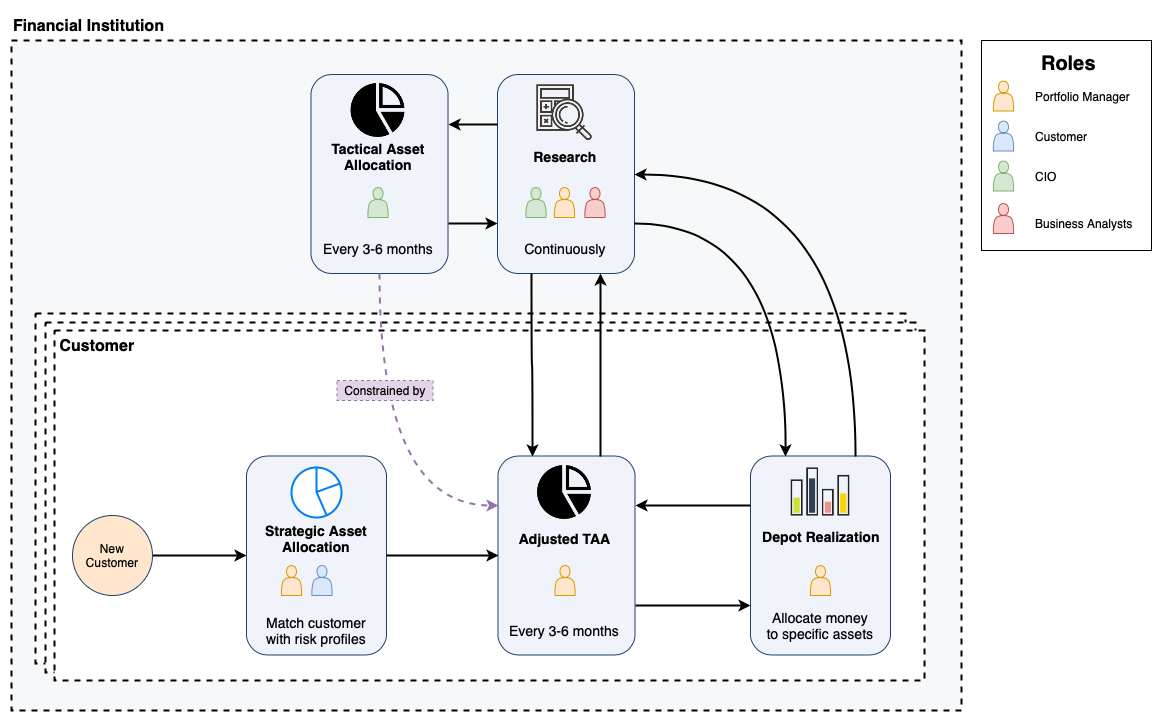
\includegraphics[scale=0.35]{img/work_model_process.png}
\end{center}

Additionally, a number of relevant observations made by the authors as well as the seminar conductors and feedbacks from the participants during the three sessions is depicted – please note that in order to fully understand some of the following aspects, the reader should have seen the old version of the simulation:
\begin{itemize}
  \item \textbf{General:} Generally, the participants enjoyed playing the game and regard it as helpful to deepen their theoretical knowledge for example from the lecture ''Asset Management: Investments'' for Bachelor students. However, they regard the system as outdated and provided the authors with various ideas and critics. Decision data for a starting period 0 will be filled out by participants in Excel for starting position before the seminar, afterward they will be saved onto the USB drives for all teams by the seminar conductors. The seminar conductors will let the market model run and save its outcome back on the USB drive. This process is time-consuming and error-prone. In general, the participants think that it is difficult to make a decision in the first round, as too few information is available. More easily accessible comparative figures for the previous year would be helpful. Additionally, the stock selection is based on insufficient knowledge about the different titles.
  \item \textbf{Investment Process:} The given and to be kept bandwidths for the different asset class positions are not optimally placed and have to be looked up frequently. An temporary over-investment during the decision process is not possible and is always disturbed by pop-up windows.
  \item \textbf{Business Administration:} Various decisions regarding marketing, human resources as well as logistics are not very clear as especially in the beginning, the background and previous period information are not completely clear for the participants. The point here is, that a suitable level of abstraction has to be chosen as on the one hand, not every decision that has to be made in reality can be implemented in such a simplified simulation. On the one hand, a suitable number of decisions have to be enabled in order to support an appropriate learning effect.
  \item \textbf{Report:} The reports provided after each round of the game load very slowly and the comparison to other teams is cumbersome. It would be helpful, if not only one group member can have the simulation and the reports on their screen. In general, more graphics are desired for a better visualization of key aspects.
  \item \textbf{Teamwork:} The enabling of a collaboration on several laptops within a team was mentioned many time. With the today’s web-based technologies, much more implementation options are available.
\end{itemize}

The observation of the different players – students and practitioners, investment beginners and experts – allowed the project team to sense, what the strengths and weaknesses of the old game are. Further, it helped to define an impact direction for the new game being developed, which resulted in another work model describing the process of the game based on its different phases. % TODO more about customer types etc.

\begin{center}
  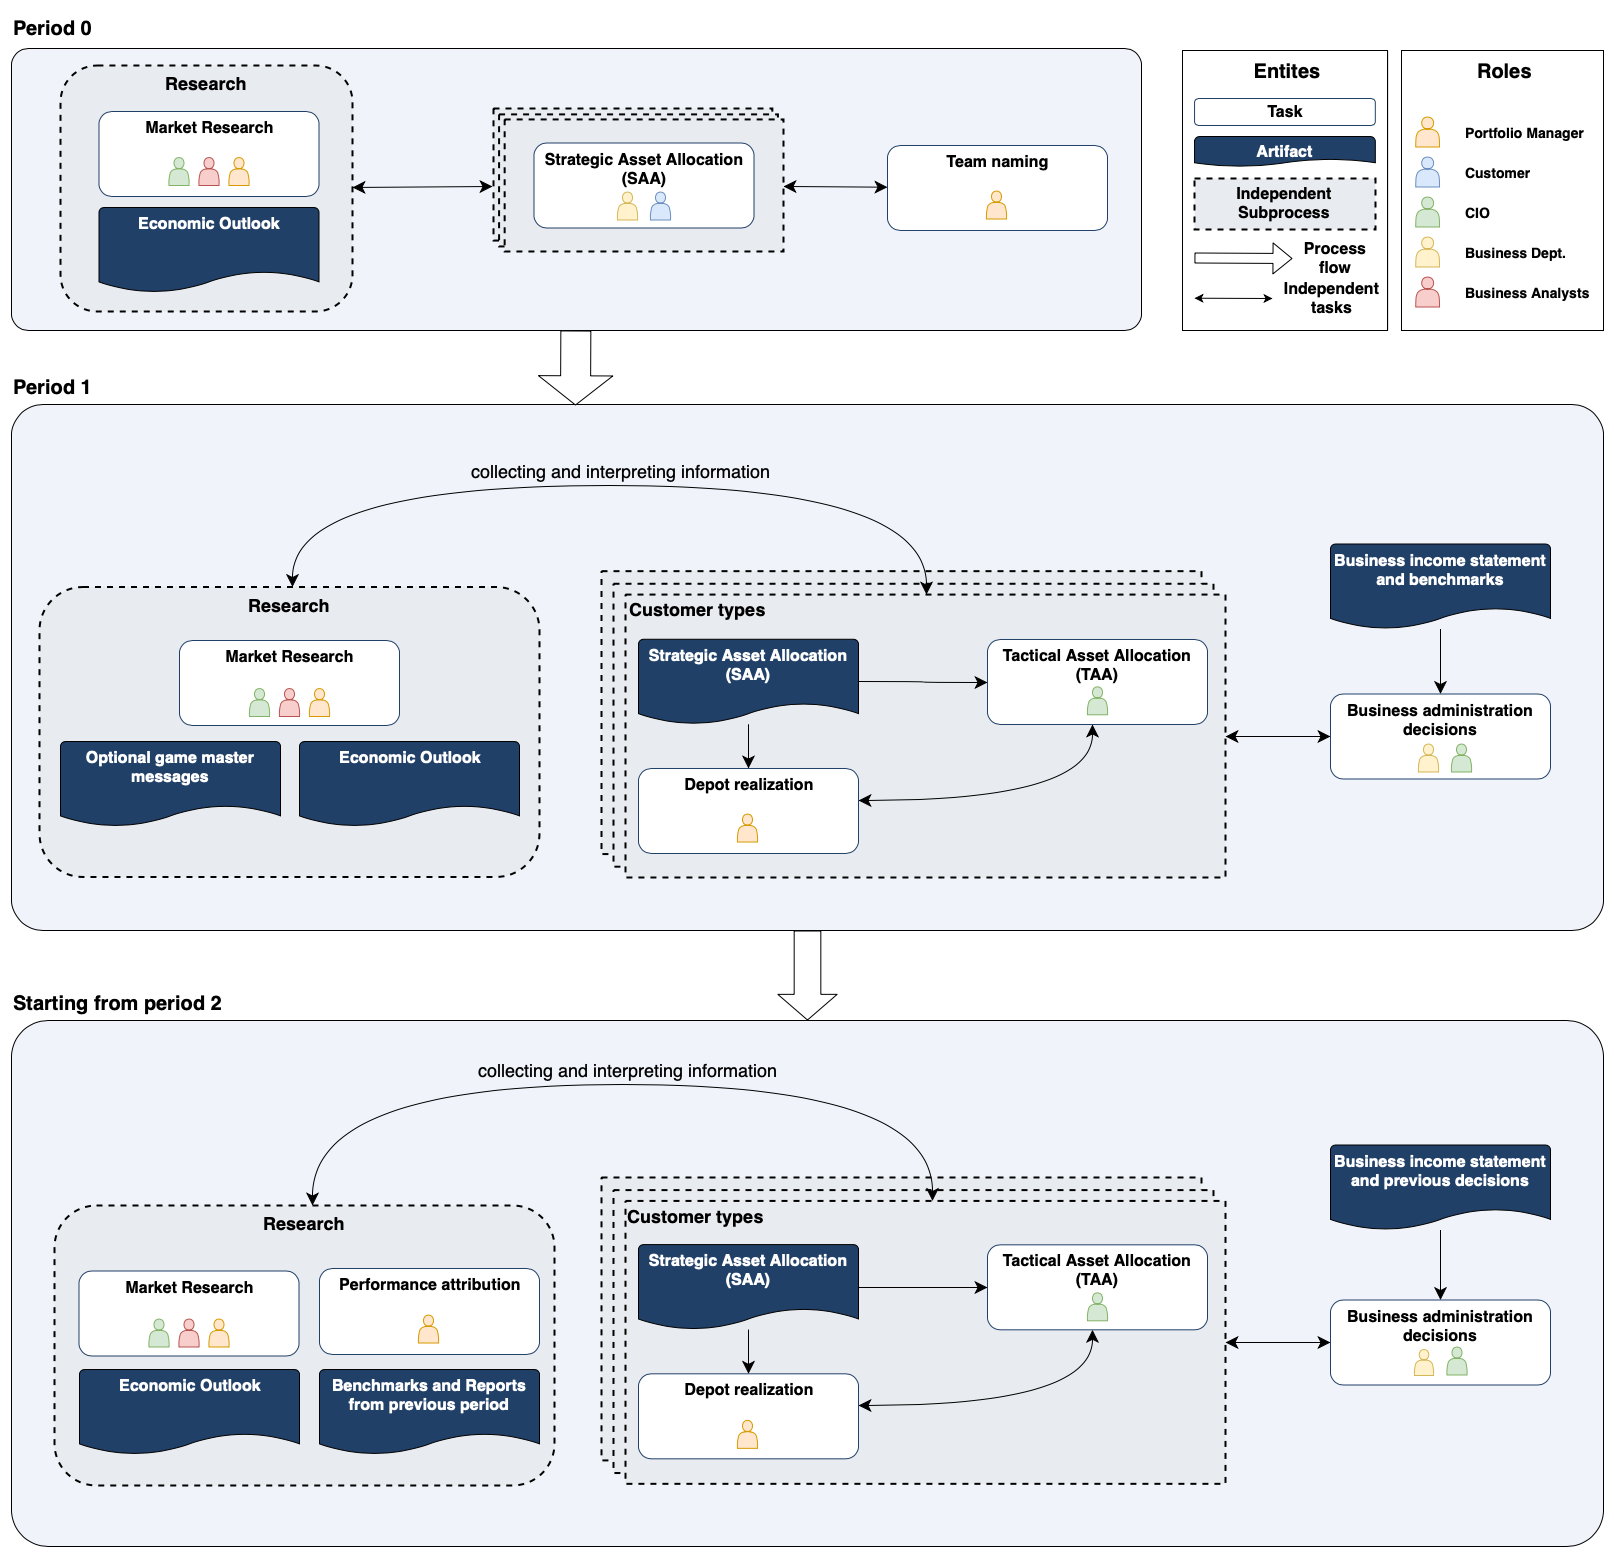
\includegraphics[scale=0.25]{img/work_model_pfm_game.png}
\end{center}

\subsection{Design and Iterative Prototyping}
Initially the authors designed multiple screens based on the predefined work model. Using a sketching software the basic screens for the students process which includes the SAA, TAA, depot relization and business administration were prototyped. As the team realized that the game does not only consist of screens from a student persepctive they decided, due to time constraints, to start implementing screens by iterative prototyping. \\

Multiple concepts had to be defined, such as how to model the game session management.
% TODO more
